\section*{Section A}
\label{sec:Section A}
\FloatBarrier % Now figures cannot float above section title


In this section, the Young's modulus of two materials 
(mild steel and aluminium) can be calculated from experimental data.

A total of six groups of data were obtained from the experiment. (See Table \ref{t1})

\subsection*{Analysis}

By plotting these 6 groups of data on a scatter plot and performing 
regression analysis, a total of 6 groups of graphs were obtained. (See Figure \ref{f1})

The Free-body-diagram of the components is shown in Figure \ref{ff1}.

\begin{figure}
    \centering
    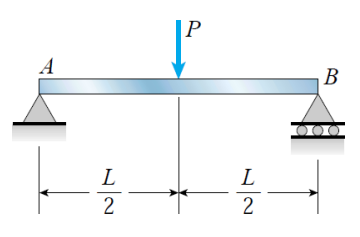
\includegraphics[]{./fig/1.png}
    \caption{Free-body-diagram}
    \label{ff1}
\end{figure}

\begin{figure}
    \centering
    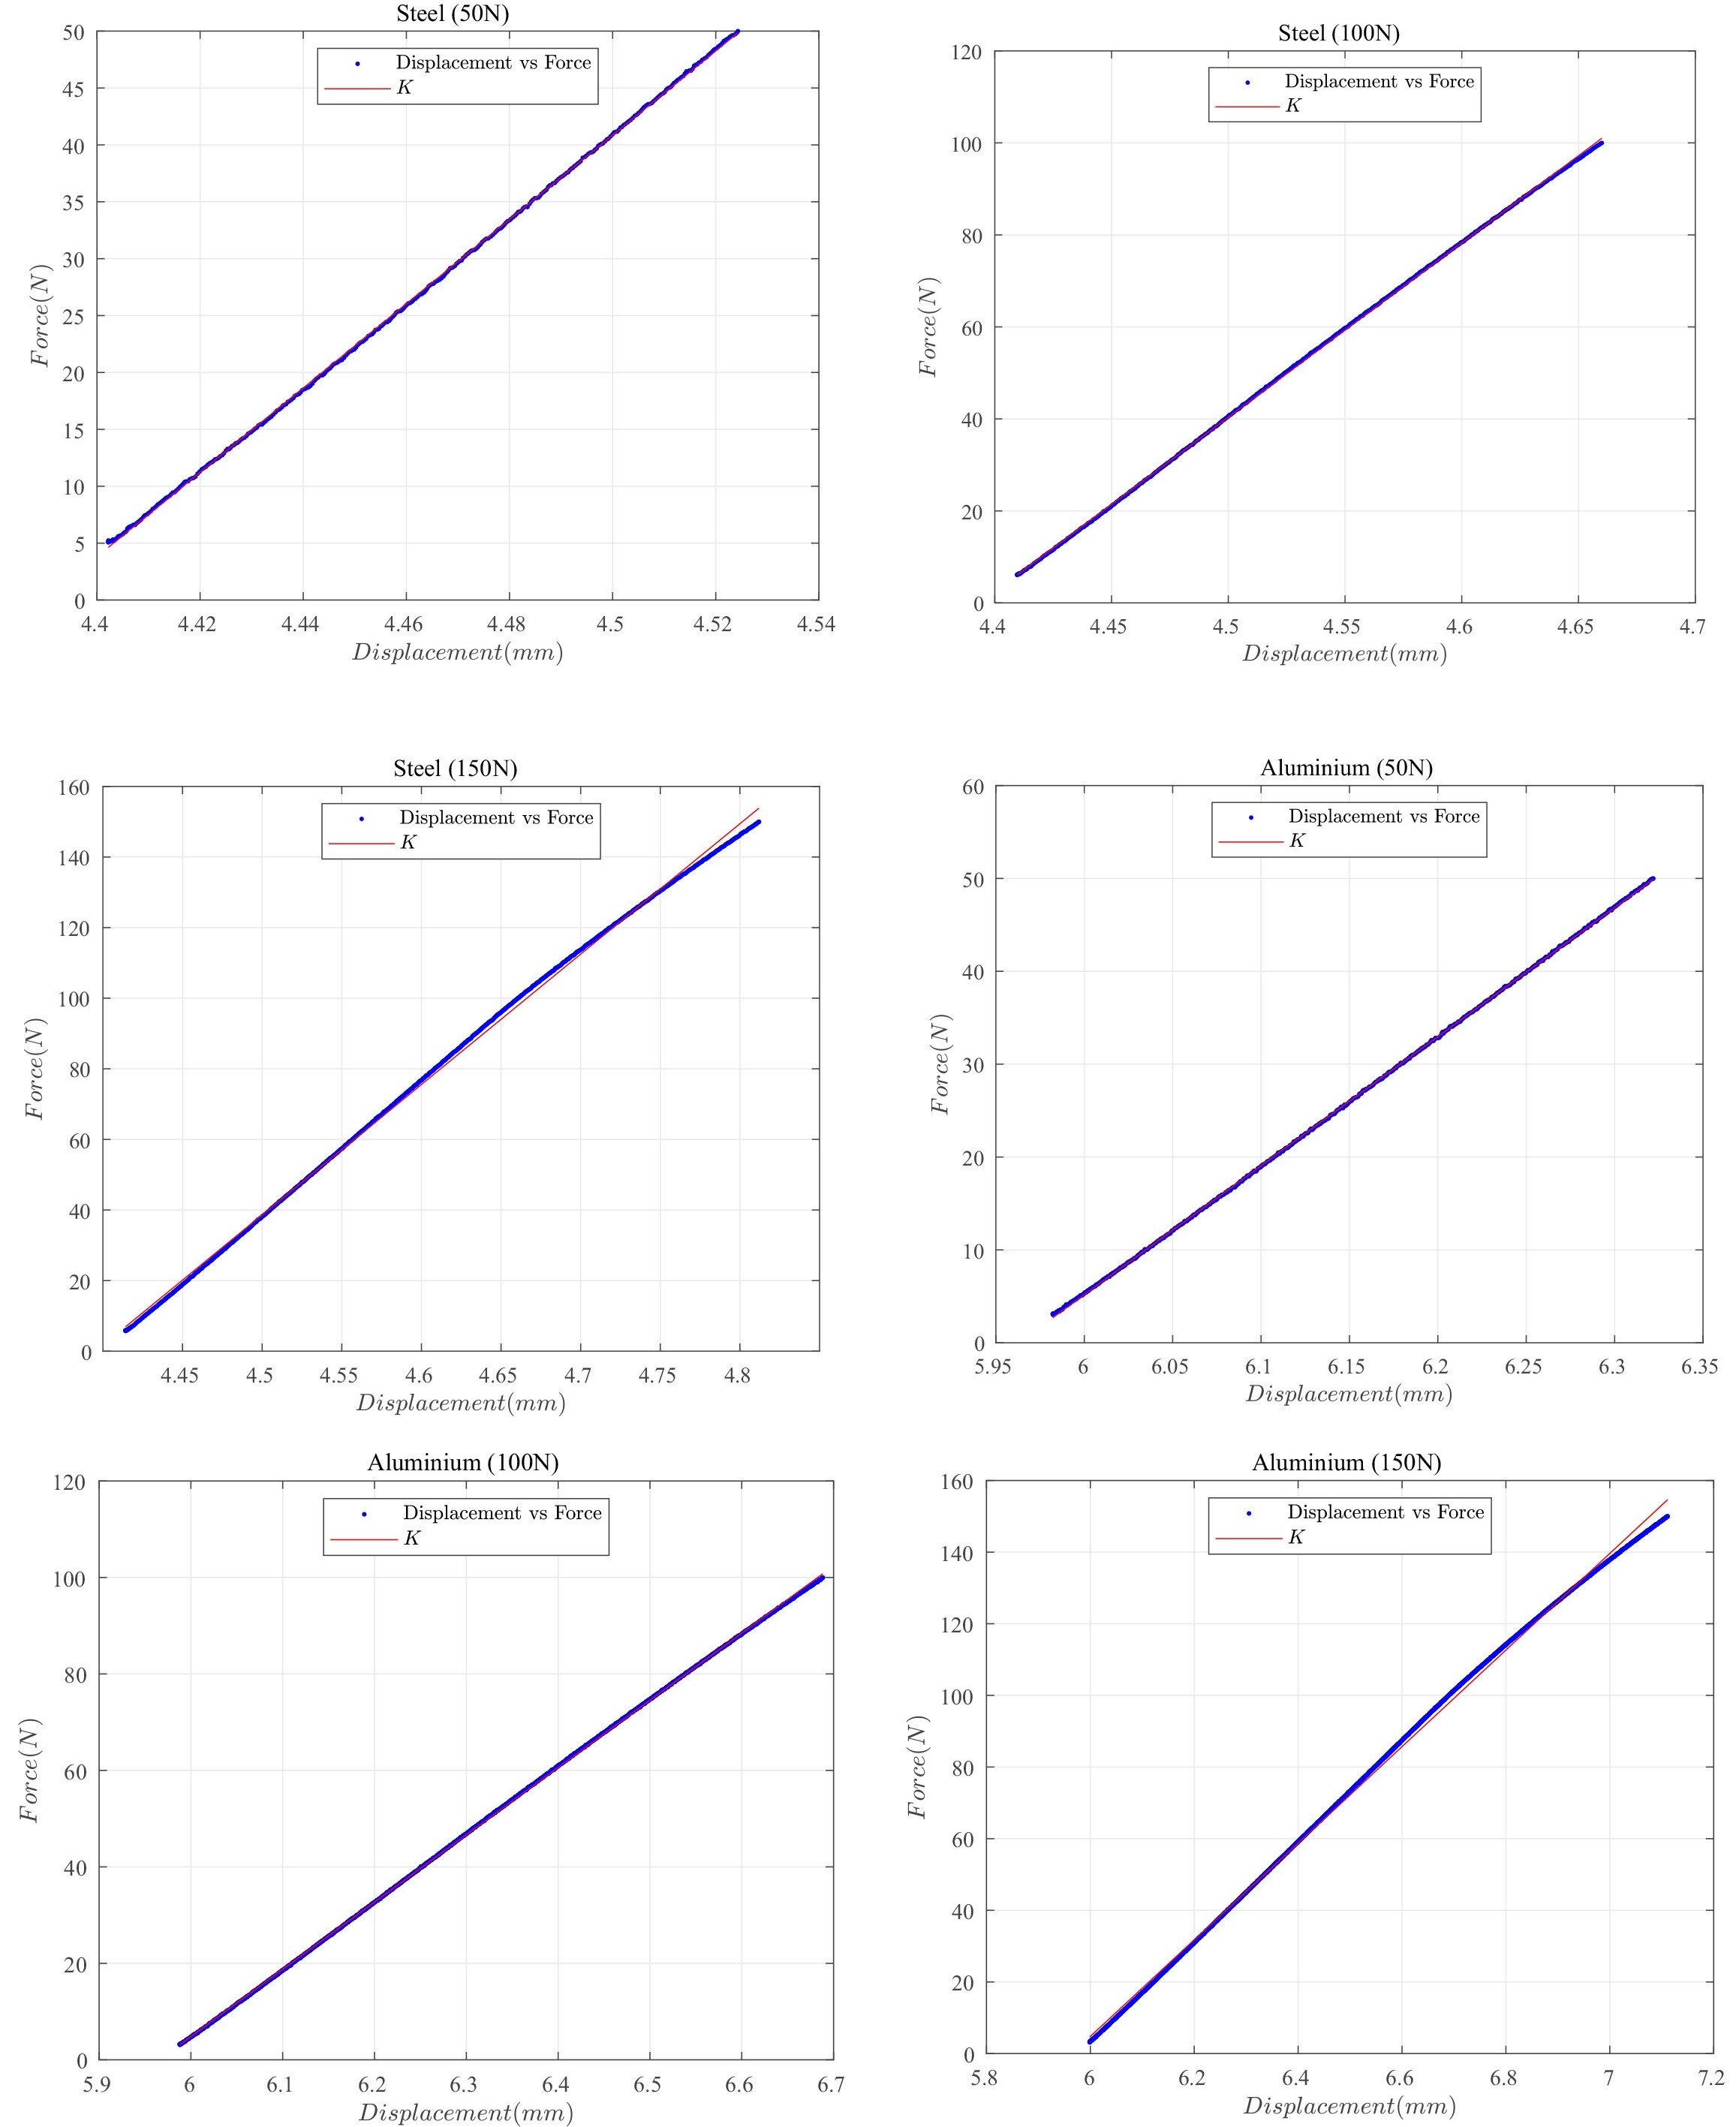
\includegraphics[width=15cm,height=21.5cm]{./fig/mix.jpg}
    \caption{Figure of linear regression analysis}
    \label{f1}
\end{figure}

\begin{minipage}[h]{\textwidth}
    \makeatletter\def\@captype{table}
    \centering
    \scalebox{1}{
    \begin{tabular}{lllll} 
        \hline
        No.  & Material    & Final load (N) &K(Slope)& R-square    \\ \hline
        1 & Steel     & 50   &370.4& 0.9999\\
        2 & Steel      & 100  &379.1& 0.9998\\
        3 & Steel      & 150   &369.4& 0.9989\\
        4 & Aluminium     & 50  &138.9& 0.9999\\
        5 & Aluminium    & 100   &139.4& 0.9999\\
        6 & Aluminium & 150   &134.8& 0.9987\\ \hline          
    \end{tabular}} 
    
    (Notice: The unit of K is N/mm, it needs to multiply $10^3$ to transfer to N/m)
    \caption{Experimental data and linear regression results}
    \label{t1} 
\end{minipage}

In order to calculate E, the moment of inertia I needs to be calculated first.

\begin{equation} 
I=\frac{bh^3}{12}=\frac{20*3^3}{12}*10^{-12}=4.5*10^{-11} (mm^4)
\end{equation}

We know 
\begin{equation} 
    \delta_{max}=\frac{PL^3}{48EI}
\end{equation}

And the slope of the regression analysis is
\begin{equation} 
    K=\frac{P}{\delta}=\frac{48EI}{L^3}
\end{equation}

So
\begin{equation} 
    E=(\frac{P}{\delta})*\frac{L^3}{48I}=K*\frac{L^3}{48I}
\end{equation}

Calculate each group of data and obtain the table \ref{t2}.

\begin{minipage}[htbp]{\textwidth}
    \makeatletter\def\@captype{table}
    \centering
    \scalebox{1.1}{
    \begin{tabular}{lll} 
        \hline
        Modulus of Elasticity  & Mild Steel    & Aluminium     \\ \hline
        $E_1(P=50N)$ & 171.482     & 64.3056    \\
        $E_2(P=100N)$ & 175.509     & 64.5370   \\
        $E_3(P=150N)$ & 171.019     & 62.4074   \\
        $E_{exp}=(E_1+E_2+E_3)/3$ & 172.670 & 63.75   \\ \hline          
    \end{tabular}} 
    
    (Unit: GPa)
    \caption{Experimental results - Modulus of elasticity}
    \label{t2} 
\end{minipage}


\subsection*{Summary}

As can be seen from the data in Table \ref{t2}, 
the modulus of elasticity of mild steel (172.67GPa) is much larger than aluminium (63.75GPa).
In addition, due to the difference in modulus of elasticity, the deformation of aluminium is 
greater than that of mild steel under the same force.

The comparison for each material indicates that there is a slight difference 
in the modulus of elasticity, 
which may be due to experimental error, and the more accurate 
modulus of elasticity can be obtained through more 
experiments.
